% !TeX spellcheck = da_DK
\section{Pilotforsøg}
Det er nødvendigt at vide hvilke frekvenser af signalet der er støj, før systemet kan designes. Grunden til dette er, at signalet skal aktivere komponenter senere i systemet og skal derfor være uden støjsignaler for ikke at påvirke outputtet. For at undgå dette frafiltreres støjsignaler. Derudover er det nødvendigt at vide, hvilket outputsignal accelerometeret giver ift. den valgte hældningsgrad. Ud fra disse oplysninger er det muligt at designe de enkelte blokke i systemet.% Oplysningerne findes på baggrund af et pilotforsøg. 

\subsection{Formål med pilotforsøg}
\begin{enumerate}
\item Identificere de frekvenser, der udgør støj i outputsignalet fra accelerometeret.
\item Identificere accelerometerets g-påvirkning ved $8^{\circ}$ og $13^{\circ}$.
\item Identificere maksimum og minimum outputsignal af accelerometeret.
\item Kontrollere om offset og sensitivitets værdierne fra databladet på accelerometeret stemmer overens med målt data.
\end{enumerate}

\subsection{Materialer}
\begin{itemize}
\item ADXL335 accelerometer.
\item To stk. 0,1 $\mu$ F kondensatorer.
\item Ledninger.
\item Breadboard.
\item 5V strøm fra spændingsforsyning.
\item NI USB-6009.
\item USB isolator USI-01.
\item Computer med ScopeLogger og MATLAB R2015a.
\item Hæftemasse.
\item Vinkelmåler
\item Lineal.
\item Tush.
\end{itemize}

\subsection{Metode}
Støjfrekvenserne i outputsignalet identificeres ved først at måle en baseline ved $0$g dvs. uden hældning. Dette medfører at signalet kan analyseres uden nogen påvirkning på outputsignalet. Dernæst måles en påvirkningen ved $1$g, hvilket svarer til en hældning på 90$^{\circ}$. Dette måles både til højre og venstre. Derved kan det sammenlignes, om der er støj ift. baseline. Det samme gøres for de specificerede hældningsgrader, som er $8^{\circ}$ og $13^{\circ}$. For at simulere den påvirkning accelerometeret udsættes for og identificere den mulige støj ved en rotation. Dette gøres ved en langsom rotation fra $0^{\circ}$ til $90^{\circ}$ til både højre og venstre. Denne metode vil også identificere minimum og maksimum outputsignal, som accelerometeret kan afgive, samt kontrollere om informationerne fra accelerometerets datablad stemmer overens med det målte data.

\subsection{Forsøget}
\textbf{Opsætning}\\
Der ses et billede af den samlede opsætningen på \figref{pforsoeg1}.
\begin{itemize}
\item Accelerometeret tilkobles breadboardet.
\item To kondensatorer på $0.10 \mu F$ tilkobles breadboardet. \fxnote{Den som sidder på pin 1 og 2 i accelerometeret fjerner støj fra strømforsygningen, mens kondensatoren fra pin 3 giver en båndbredde på 50 Hz.}
\item Accelerometeret tilnyttes en forsyningsspænding på 5V.
\item Outputtet fra systemet sendes igennem NI USB-6009.
\item Signalet fra NI USB-6009 sendes igennem USI-01. \fxnote{USB isolator}
\item Outputsignalet fra USI-01 sendes ind i computeren, hvor det optages med ScopeLogger og behandles i MATLAB R2015a.
\end{itemize}

\begin{figure}[H]
	\centering
	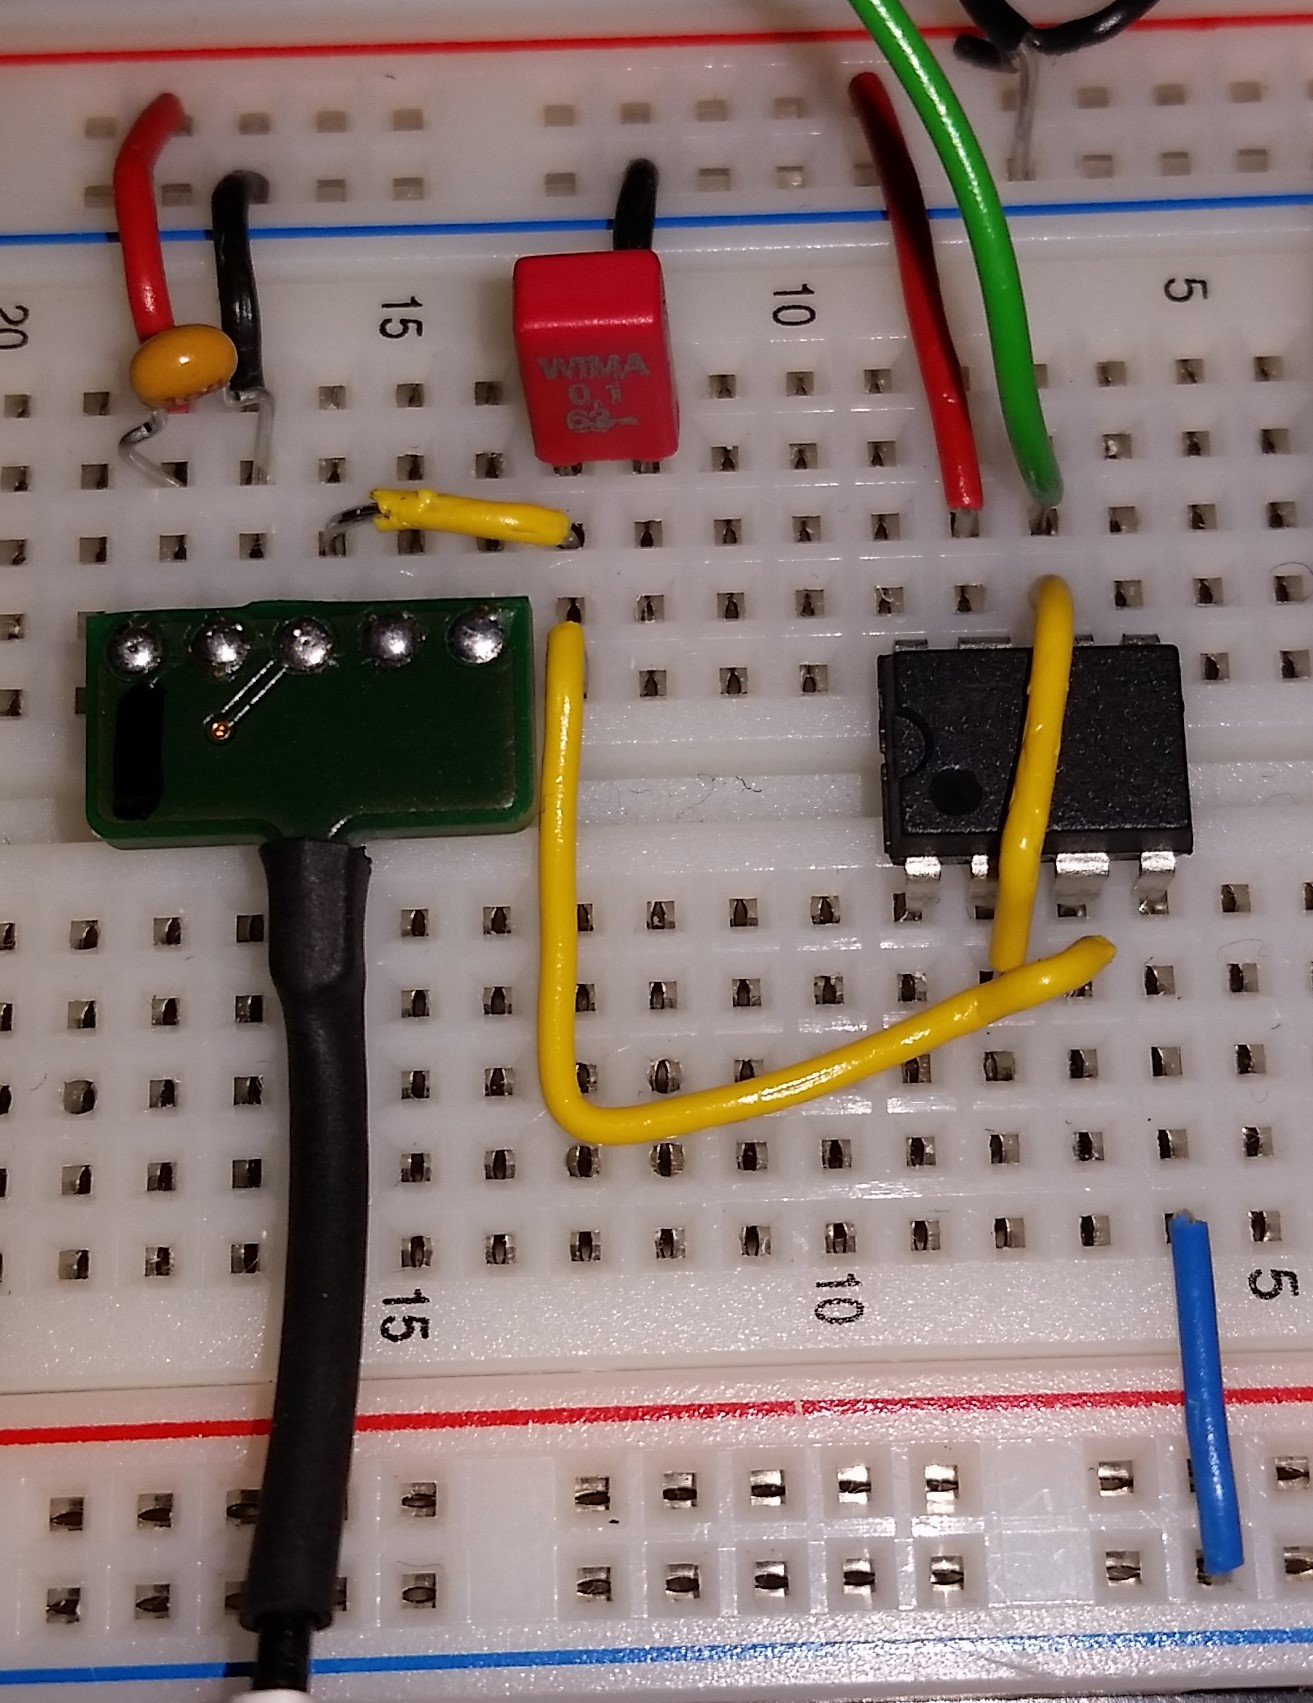
\includegraphics[scale=0.15]{figures/cProblemloesning/PF2.jpg}
	\caption{På billedet ses opsætningen på breadboardet. De røde ledninger symboliserer inputtet fra den 5V strømforsyning. De sorte ledninger fungerer som ground. Den gule ledning fungerer som en leder for outputtet fra accelerometerets pågældende akse (kan skiftes imellem række 15, 16 og 17 alt efter hvilken akse, der skal måles på). Den grønne ledning symboliserer outputtet fra breadboardet, som sendes til NI USB-6009.}
	\label{pforsoeg1}
\end{figure}

\noindent\textbf{Fremgangsmåde}\\
Hele pilotforsøgets opsætning ses på \figref{pforsoeg2}. \\
Accelerometeret sættes fast med hæftemasse på en lineal så der måles på x-aksen, når der sker en rotation til højre og venstre. Vinkelmåleren sættes fast i en lodret position, så linealen kan følge graderne. Herved bliver $90^{\circ}$ på vinkelmåleren accelerometerets nulpunkt. \\
Først måles baseline for 0g og 1g i 30 sekunder. Dette gøres ved, at linealen med accelerometeret holdes i 30 sekunder ved nulpunktet samt $90^{\circ}$ til henholdsvis højre og venstre. Dette giver 3 baselines, som optages og gemmes i ScopeLogger. Herudover måles en baseline for g påvirkningen af accelerometeret ved $8^{\circ}$ og $13^{\circ}$. Dette gøres ved at holde accelerometeret i 30 sekunder på $8^{\circ}$ og $13^{\circ}$ henholdsvis til højre og venstre. Herved fås 4 baselines, som optages og gemmes i ScopeLogger.
Til sidst måles g påvirkningen af accelerometeret under rotation fra $0^{\circ}$ til $\pm$ $90^{\circ}$ for både højre og venstre. Her måles 10 sekunders baseline inden og efter rotationen, som varer 10 sekunder og foretages langsomt og kontrolleret. Disse to målinger optages og gemmes ligeså i ScopeLogger. \\
Alt data vil efterfølgende blive behandlet i MATLAB R2015a, hvor der beregnes en gennemsnitsværdi for de syv baselines samt foretages en Fast Fourier Transformation (FFT) på samtlige målinger. FFT foretages for at få en repræsentation af støj på signalet. Ved baselines kan man se, hvilken påvirkning omgivelserne har på signalet, da der ikke er nogen bevægelse på dette signal.

\begin{figure}[H]
	\centering
	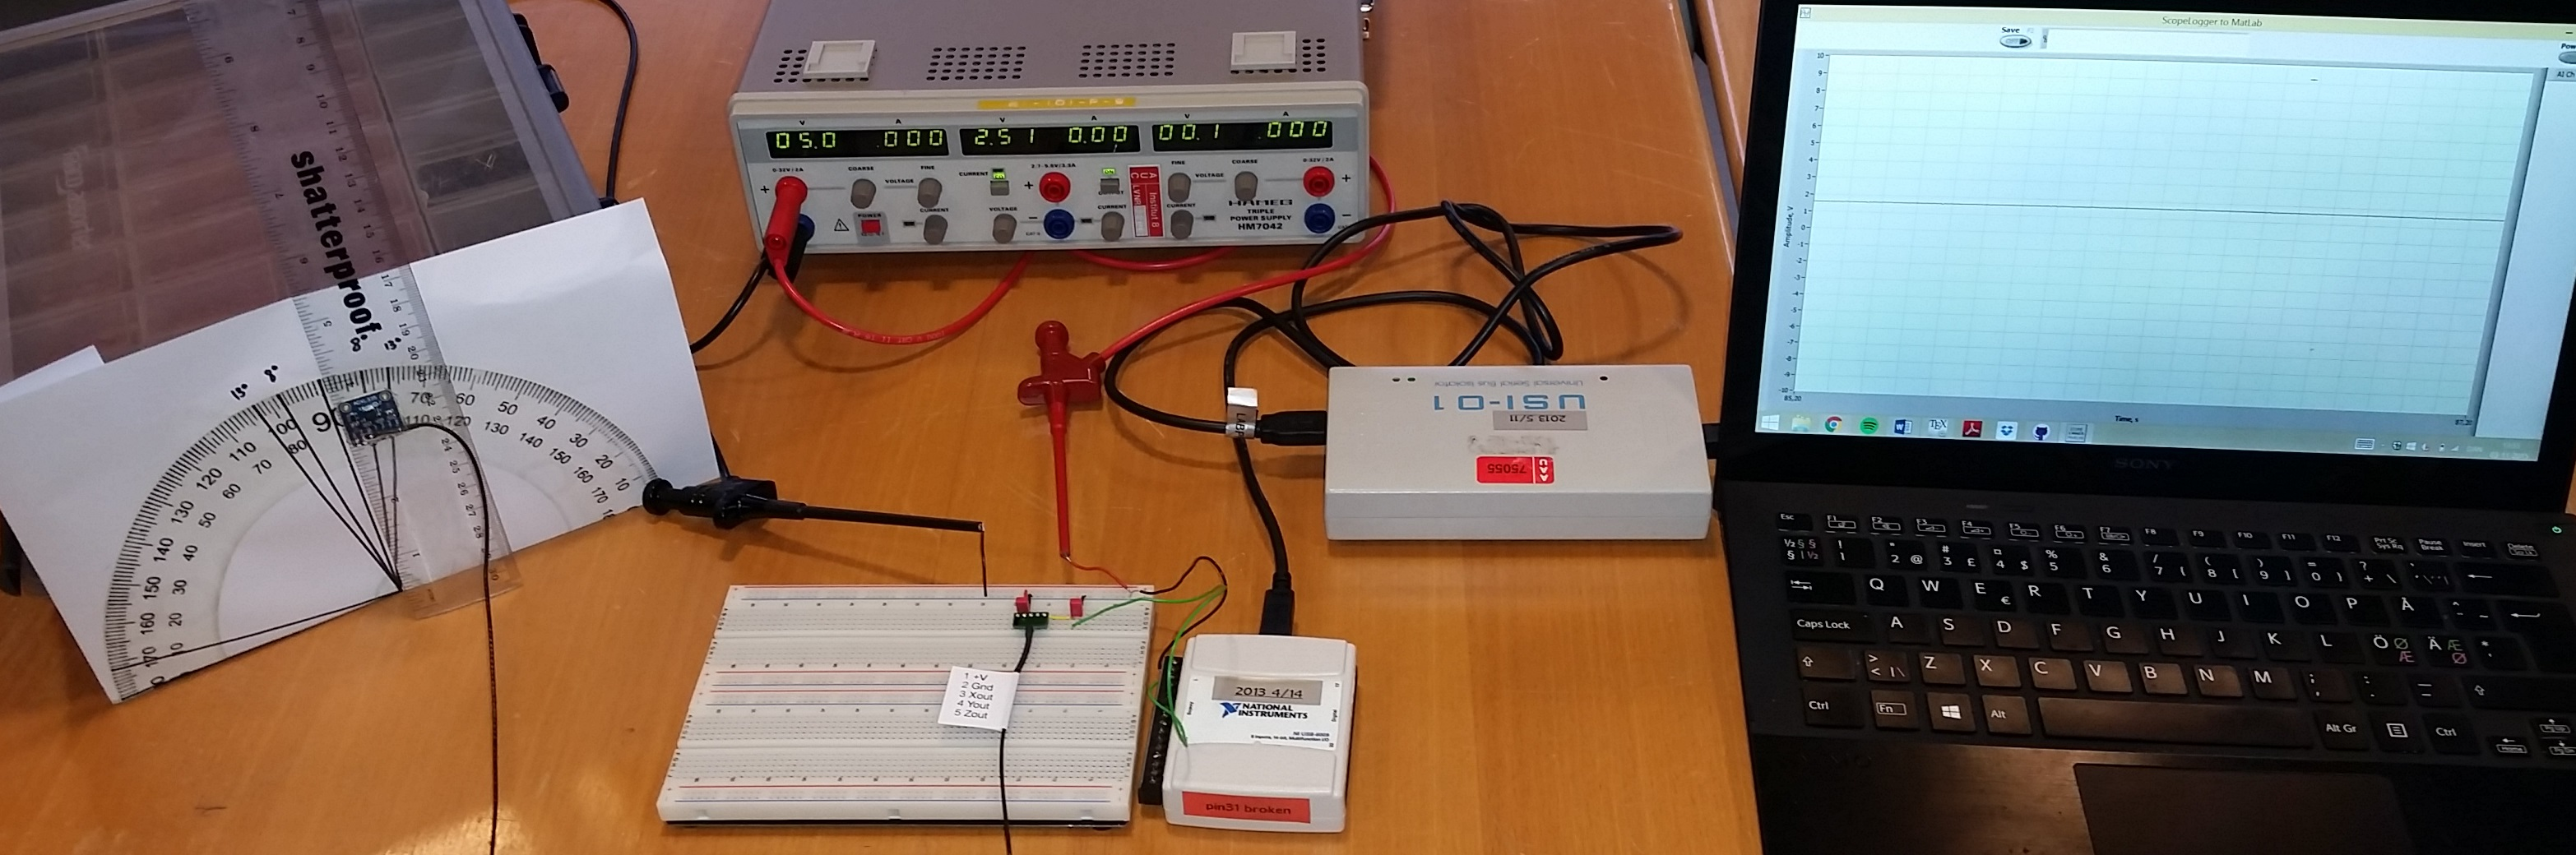
\includegraphics[scale=0.14]{figures/cProblemloesning/Pilotforsoeg1.jpg}
	\caption{På billedet ses (fra venstre til højre) opsætningen af accelerometeret på linealen, der kan aflæse grader på vinkelmåleren. Øverst i midten på billedet ses den 5V spændingsforsyning, som leder strømmen til- og ground fra breadboardet. Nederst i midten ses breadboardet, der sender sit output videre til NI USB-6009. Herefter ledes signalet igennem USI-01 og til sidst ind i computeren, hvor det optages i ScopeLogger.}
	\label{pforsoeg2}
\end{figure}


\subsection{Databehandling}
\subsubsection{Støj}

\subsubsection{Accelerometers påvirkning}
\subsubsection{Outputsignal}

\subsubsection{Databladet}